\documentclass[border=10pt]{standalone}
\usepackage{tikz}
\usepackage{pgfplots}
\usepackage{amssymb}
\pgfplotsset{compat=1.18}

\begin{document}
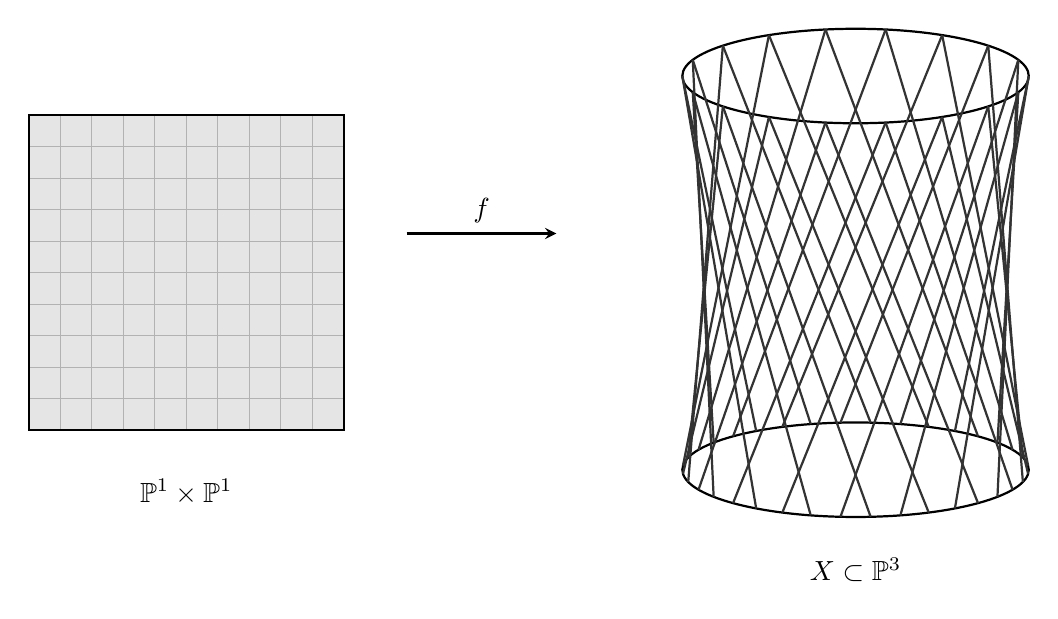
\begin{tikzpicture}

% === Left: P^1 x P^1 as a grid ===
\begin{scope}[shift={(-5,0)}]
  % Filled square
  \fill[gray!20] (-2,-2) rectangle (2,2);
  % Grid lines
  \foreach \i in {-2,-1.6,...,2} {
    \draw[gray!60] (\i,-2) -- (\i,2);
    \draw[gray!60] (-2,\i) -- (2,\i);
  }
  \draw[thick] (-2,-2) rectangle (2,2);
  \node[below] at (0,-2.5) {$\mathbb{P}^1 \times \mathbb{P}^1$};
\end{scope}

% === Arrow ===
\draw[->,thick,>=stealth] (-2.2,0.5) -- (-0.3,0.5) 
  node[midway,above] {$f$};

% === Right: Quadric surface (hyperboloid) via rulings ===
\begin{scope}[shift={(3.5,0)}]
  % Draw two families of rulings on a hyperboloid
  % Parametrize: x = cosh(v)cos(u), z = cosh(v)sin(u), y = sinh(v)
  
  % Top ellipse
  \draw[thick] (0,2.5) ellipse (2.2 and 0.6);
  % Bottom ellipse
  \draw[thick] (0,-2.5) ellipse (2.2 and 0.6);
  
  % First family of rulings
  \foreach \a in {0,20,...,340} {
    \pgfmathsetmacro{\xt}{2.2*cos(\a)}
    \pgfmathsetmacro{\zt}{0.6*sin(\a)}
    % Connect to rotated point on bottom ellipse
    \pgfmathsetmacro{\b}{\a+55}
    \pgfmathsetmacro{\xb}{2.2*cos(\b)}
    \pgfmathsetmacro{\zb}{0.6*sin(\b)}
    \draw[thick,black!80] (\xt,{2.5+\zt}) -- (\xb,{-2.5+\zb});
  }
  
  % Second family of rulings
  \foreach \a in {0,20,...,340} {
    \pgfmathsetmacro{\xt}{2.2*cos(\a)}
    \pgfmathsetmacro{\zt}{0.6*sin(\a)}
    \pgfmathsetmacro{\b}{\a-55}
    \pgfmathsetmacro{\xb}{2.2*cos(\b)}
    \pgfmathsetmacro{\zb}{0.6*sin(\b)}
    \draw[thick,black!80] (\xt,{2.5+\zt}) -- (\xb,{-2.5+\zb});
  }
  
  \node[below] at (0,-3.5) {$X \subset \mathbb{P}^3$};
\end{scope}

\end{tikzpicture}
\end{document}